\documentclass[a4paper]{article}

\usepackage[margin=1in]{geometry} 
\usepackage{amsmath,amsthm,amssymb}
\usepackage{amssymb}
\usepackage{float}
\usepackage{graphicx}
\usepackage{xcolor}
\usepackage[UKenglish]{isodate}
\origdate
\cleanlookdateon
\usepackage[utf8]{inputenc}
\usepackage[hidelinks]{hyperref}
\usepackage{tikz-cd}
\usepackage{enumitem}
\usepackage{mathtools}
\usepackage{pgfplots}
\usepackage{float}
\usepackage{tikz, venndiagram}
\usepackage{tkz-euclide}
\usepackage{tabu}
\renewcommand{\baselinestretch}{1.5} 

%%% Better lambda 
\usepackage{pifont}
\makeatletter
\newcommand\Pimathsymbol[3][\mathord]{%
  #1{\@Pimathsymbol{#2}{#3}}}
\def\@Pimathsymbol#1#2{\mathchoice
  {\@Pim@thsymbol{#1}{#2}\tf@size}
  {\@Pim@thsymbol{#1}{#2}\tf@size}
  {\@Pim@thsymbol{#1}{#2}\sf@size}
  {\@Pim@thsymbol{#1}{#2}\ssf@size}}
\def\@Pim@thsymbol#1#2#3{%
  \mbox{\fontsize{#3}{#3}\Pisymbol{#1}{#2}}}
\makeatother
% the next two lines are needed to avoid LaTeX substituting upright from another font
\input{utxmia.fd}
\DeclareFontShape{U}{txmia}{m}{n}{<->ssub * txmia/m/it}{}
% you may also want
\DeclareFontShape{U}{txmia}{bx}{n}{<->ssub * txmia/bx/it}{}
% just in case
%\DeclareFontShape{U}{txmia}{l}{n}{<->ssub * txmia/l/it}{}
%\DeclareFontShape{U}{txmia}{b}{n}{<->ssub * txmia/b/it}{}
% plus info from Alan Munn at https://tex.stackexchange.com/questions/290165/how-do-i-get-a-nicer-lambda?noredirect=1#comment702120_290165
\newcommand{\pilambdaup}{\Pimathsymbol[\mathord]{txmia}{21}}
\pgfplotsset{compat=1.16}
\begin{document}
\title{Midterms Revision Guide\\[0.1cm]
    \large 30.003 Probability and Statistics, Term 4 2019}
\author{Wei Min Cher}
\date{05 Jan 2020}

\maketitle

\tableofcontents

\newpage
\section{W1: Probability and Statistics}
\subsection{Definitions}
\begin{itemize}
    \item Population: well defined collection of objects
    \item Sample: subset of population selected in certain manner
    \item Variable: any characteristic whose value may change from one object to another in population
    \newline
    \item Probability: properties of populations known, question regarding sample taken from population are investigated \textbf{(deductive reasoning)}
    \item Statistics: characteristics of sample known from experiments, conclusions regarding population are made \textbf{(inductive reasoning)}
\end{itemize}
\begin{center}
    \begin{tikzcd}
    \text{Population} \arrow[r, bend left=45, "\text{Probability}"{name=U, above}]
    & \text{Sample} \arrow[l, bend left=45, "\text{Statistics}"{name=D}]
    \end{tikzcd}
\end{center}
\subsection{Frequency} 
\begin{itemize}
    \item Frequency: number of times value occurs in data set
    \item Relative frequency: fraction or proportion of times the value occurs
\end{itemize}
\subsection{Range and mean}
\begin{itemize}
    \item Range: difference between largest and smallest sample values
    \item Mean: average of all values
    \newline
    \item Population mean is denoted by $\mu$
    \item Sample mean is denoted by $\Bar{x}$, where $$\Bar{x} = \frac{\sum x_{i}}{n}, \text{ and $n$ denoting the number of data points}$$
\end{itemize}
\subsection{Variance and standard deviation}
\begin{itemize}
    \item Variance: measures variability of data set
    \item Population variance is denoted by $\sigma^2$, where
    $$\sigma^2 = \frac{1}{N}\sum_{i=1}^{N}\left(x_{i}-\mu\right)^{2}, \text{ and $N$ denoting the size of the population}$$
    \item Sample variance is denoted by $s^2$, where
    $$s^2 = \frac{1}{n-1}\sum_{i=1}^{n}\left(x_{i}-\Bar{x}\right)^2, \text{ and $n$ denoting the size of the sample}$$
    \newline
    \item Standard deviation is denoted as $\sigma$ for population variance and $s$ for sample variance, and is calculated either by:
    $$\sigma = \sqrt{\sigma^2}, \text{ or } s = \sqrt{s^2}$$
    where $\sigma^2$ is the population variance and $s^2$ is the sample variance
    \begin{itemize}[label=$\circ$]
        \item Shortcut to calculate population variance:
        $$\sigma^2 = \frac{1}{N}\sum_{i=1}^{N}x_{i}^{2}-\mu^2$$
    \end{itemize}
\end{itemize}
\subsection{Median}
\begin{itemize}
    \item Median: the middle value in a data set
\end{itemize}
\subsection{Percentile}
\begin{itemize}
    \item value below which a given percentage of observations falls
    \item data set is ordered as $x_{1}' \leq x_{2}'\leq \cdots \leq x_{n}'$,\\ where $x_{1}'$ and $x_{n}'$ are the smallest and largest data values respectively
    \item $x_{i}'$ corresponds to the $\frac{100(i-0.5)}{n}$th percentile
\end{itemize}
\subsection{Sample space and events}
\begin{itemize}
    \item Sample space: the set of all possible outcomes of an experiment
    \begin{enumerate}
        \item Collectively exhaustive
        \item Mutually exclusive
    \end{enumerate}
    \item Event: collection of outcomes contained in sample space $\Omega$
    \begin{enumerate}
        \item Simple event: exactly one outcome
        \item Compound event: \textgreater \ 1 outcome
    \end{enumerate}
\end{itemize}
\subsection{Sample Space vs Population}
\begin{itemize}
    \item Sample space: contains mutually exclusive events
    \item Population: events can repeat many times
\end{itemize}
\subsection{Set Theory}
\begin{itemize}
    \item Null event, $\varnothing$: event with no outcome
    \item Events A and B are mutually exclusive/disjoint if $A\cap B = \varnothing$
\end{itemize}
\subsection{De Morgan's Laws}
\begin{align*}
    (A\cup B)^{c} &= A^{c} \cap B^{c}\\
    (A\cap B)^{c} &= A^{c} \cup B^{c}\\
    A \cup B &= A+B-A\cap B
\end{align*}
\subsection{Axiom of Probability}
\begin{enumerate}
    \item For any event A, P(A) $\leq$ 0.
    \item P($\Omega$) = 1
    \item Any infinite collection of mutually exclusive/disjoint events $A_{1}, A_{2}, A_{3}, \ldots, A_{n}$ satisfies
    $$P(A_{1}\cup A_{2}\cup A_{3} \cup \ldots \cup A_{n}) = \sum_{i=1}^{\infty}P(A_{i})$$
\end{enumerate}
\subsection{Properties of Probability}
\begin{itemize}
    \item For any event A, $P(A) + P(A^c) = 1$.
    \item $P(\Omega) = P(A\cup A^c) = P(A) + P(A^c)$\\
    $\because$ \ $A$ \text{and} $A^c$ are disjoint
    \item For any event A, $P(A) \leq 1$.
    \item For a null event $\varnothing$, $P(\varnothing) = 0$
    \begin{itemize}[label=$\circ$]
        \item Does \textbf{NOT} suggest A = $\varnothing$
    \end{itemize}
    \item Similarly, P(A) = 1 does \textbf{NOT} suggest A = $\Omega$
\end{itemize}
\subsection{Equally likely outcomes}
$$P(\text{equally likely event}) = \frac{1}{n},\text{ where n is the number of equally likely events}$$
\newpage
\section{W1: Counting Technique}
\subsection{Finding probability}
\begin{itemize}
    \item Computing probability $\rightarrow{}$ counting
    $$P(A) = \frac{N(A)}{N}$$
    \begin{itemize}[label=$\circ$]
        \item where $N(A)$ is the number of outcomes for event A, \\and $N$ is the number of outcomes in the sample space  
    \end{itemize}
\end{itemize}
\subsection{Tuple}
\begin{itemize}
    \item Group of $k$ elements: k-tuple
    \item The 1\textsuperscript{st} element is selected in $n_1$ ways;
    the 2\textsuperscript{nd} element is selected in $n_2$ ways; the k\textsuperscript{th} element is selected in $n_k$ ways; such that \textit{the elements are selected independently}.
\end{itemize}
\subsection{Permutation}
\begin{itemize}
    \item Ordered subset
    \item Number of permutations of size $k$ formed from $n$ objects:
    $$P_{k, n} = \frac{n!}{(n-k)!}$$
\end{itemize}
\subsection{Combination}
\begin{itemize}
    \item Unordered subset of a group
    \item Number of combinations of size $k$ formed from $n$ objects:
    $$\binom{n}{k} \text{ or }C_{k, n} = \frac{P_{k, n}}{k!} = \frac{n!}{k!(n-k)!}$$
    \item Disregards the different outcomes due to order
\end{itemize}
\newpage
\section{W2: Conditional Probability}
\begin{itemize}
    \item Probability of event A given that event B has occurred: P(A$\mid$B)
    $$P(A\mid B) = \frac{P(A\cap B)}{P(B)}$$
\end{itemize}
\begin{center}
    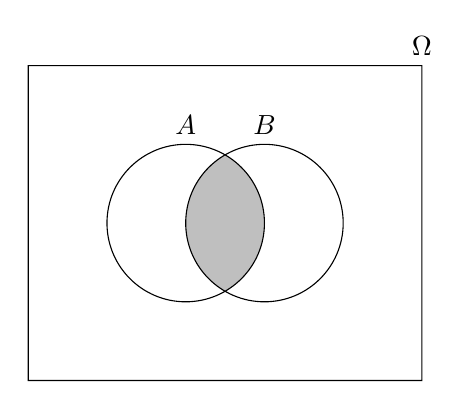
\begin{tikzpicture}
\scope % A \cap B
\clip (0,0) circle (1);
\fill[lightgray] (1,0) circle (1);
\endscope
% outline
\draw (0,0) circle (1) (0,1) node [text=black,above] {$A$}
      (1,0) circle (1) (1,1) node [text=black,above] {$B$}
      (-2,-2) rectangle (3,2) node [text=black,above] {$\Omega$};
\end{tikzpicture}
\end{center}
\subsection{Law of Total Probability}
\begin{itemize}
    \item Let $A_{1}, A_{2}, \ldots, A_{k}$ be mutually exclusive and exhaustive events.\\For any other event B,
    $$P(B) = \sum_{i=1}^{k}P(B\mid A_{i})P(A_{i})$$
\end{itemize}
\begin{center}
    \begin{venndiagram3sets}[labelA = $A_{1}$, labelB = $A_{2}$, labelC = $A_{3}$, labelABC = $B$]
    \fillACapB  
    \fillACapC
    \fillBCapC
    \fillACapCCapB
    \setpostvennhook{\draw (venn top right) node[text=black,above] {$\Omega$};}
    \end{venndiagram3sets}
\end{center}
\subsection{Bayes' Theorem}
\begin{align*}
    P(A_{j}\mid B) &= \frac{P(A_{j}\cap B)}{P(B)}\\
    &= \frac{P(B\cap A_{j})}{P(B)}\\
    &= \frac{P(B\mid A_{j})P(A_{j})}{\sum_{i=1}^{k}P(B\mid A_{i})P(A_{i})}
\end{align*}
\newpage
\subsection{Independence of Random Variables}
\begin{itemize}
    \item Independence: occurrence/non-occurrence of one event has no bearing\\ on the chance that the other will occur
    \begin{itemize}[label=$\circ$]
        \item $P(A\mid B) = P(A)$: A and B are independent
        \item $P(A\mid B) \neq P(A)$: A and B are not independent
    \end{itemize}
    \item Independence of A and B also implies $P(B\mid A) = P(B)$ if $P(A) > 0$
\end{itemize}
\subsubsection{Multiplication Rule}
\begin{itemize}
    \item A and B are independent iff. $P(A\cap B) = P(A)P(B)$
\end{itemize}
\subsubsection{Independence of several events}
    $$P(A_{i1}\cap A_{i2}\cap\ldots\cap A_{ik}) = P(A_{i1})P(A_{i2})\ldots P(A_{ik})$$
\newpage
\section{W2: Discrete Random Variable}
\subsection{Probability Mass Function (PMF) for Discrete RV}
\begin{itemize}
    \item For any pmf, $p(x)\leq 0$ and $\sum_{\text{all possible x}}p(x) = 1$
\end{itemize}
\subsection{Bernoulli RV}
\begin{itemize}
    \item pmf of any Bernoulli RV:
    $$p(x; \alpha) = \begin{cases}
    \quad 1-\alpha,&\mbox{if }x = 0\\
    \quad \alpha,&\mbox{if }x = 1\\
    \quad 0, &\mbox{otherwise}
    \end{cases}
    $$
    \item $\alpha$ is a parameter, where $0<\alpha<1$
\end{itemize}
\subsection{Bernoulli process}
\begin{itemize}
    \item A process with repeated independent trials
    \item 2 outcomes: 1 (success), 0 (failure)
    \item Success rate of trials is the same
\end{itemize}
\subsection{Binomial distribution}
\begin{itemize}
    \item pmf of binomial RV:
    $$p(x;n,p) = \begin{cases}
    \quad C_{x, n}p^{x}(1-p)^{n-x},&\mbox{}x = 0, 1, \ldots, n\\
    \quad 0, &\mbox{otherwise}
    \end{cases}
    $$
    \begin{itemize}[label=$\circ$]
        \item where $n$ is the number of trials, and $p$ is the success rate of each trial
    \end{itemize}
\end{itemize}
\subsection{Geometric distribution}
\begin{itemize}
    \item Probability distribution of number of Bernoulli trials $X$ needed to get 1 success
    \item If $X = x$, $x-1$ failures followed by success
    \item pmf of geometric RV:
    $$p(x) = \begin{cases}
    \quad p(1-p)^{x-1},&\mbox{}x = 1, 2, \ldots\\
    \quad 0, &\mbox{otherwise}
    \end{cases}
    $$
    \begin{itemize}[label=$\circ$]
        \item where $p$ is the success rate of each trial
    \end{itemize}
\end{itemize}
\subsection{Poisson distribution}
\begin{itemize}
    \item Used to model the number of occurrences of events in a time interval,\\ where the average occurrence is $\pilambdaup$
    \item pmf of Poisson RV:
    $$
    p(x; \pilambdaup) = \begin{dcases*}
    \quad\frac{\pilambdaup^{x} e^{-\pilambdaup}}{x!},&$x$ = 0, 1, $\ldots$\\
    \quad0\vphantom{\frac{0}{0}}, & otherwise
    \end{dcases*}
    $$
    \begin{itemize}[label=$\circ$]
        \item where $\pilambdaup$ is the parameter of Poisson distribution
    \end{itemize}
\end{itemize}
\subsection{Cumulative Distribution Function (CDF)}
\begin{itemize}
    \item CDF $F(x)$ of discrete RV $X$ with pmf $p(x):$
    $$F(x) = P(X\leq x) = \sum_{y: y\leq x}p(y)
    $$
    \item $F(x)$ is the probability that the observed value is at most $x$
    \item Graph of $F(x)$ for discrete RV $X$ is the linear combination of step functions, such that
    $$
    \lim_{x\to -\infty}F(x) = 0\text{ and }\lim_{x\to\infty}F(x) = 1
    $$
\end{itemize}
\newpage
\section{W3: Expectation}
\subsection{Expected Value}
\begin{itemize}
    \item Expected value $E(X)$
    $$E(X) = \mu_{x} = \sum_{x\in D}x\cdot p(x), \text{ provided that }\sum_{x \in D}|x|\cdot p(x) < \infty
    $$
    \item Expected value of a function $E[h(X)]$
    $$E[h(X)] = \mu_{h(x)} = \sum_{x\in D}h(x)\cdot p(x)
    $$
    \item Expected value of a linear function $aX + b$
    $$E(aX+b) = aE(X) + b
    $$
\end{itemize}
\subsection{Variance}
\begin{itemize}
    \item Variance $V(X)$
    \begin{center}
        $\begin{matrix}
        V(X) = \sum_{x\in D}(x-\mu)^{2}p(x) = E[(X-\mu)^2], \text{ provided that the expectation exists}\\
        \textbf{OR}\\
        \text{Population variance, }\sigma^2 = V(X) = E(X^2)-[E(X)]^2
        \end{matrix}$
    \end{center}
    \item Variance of a function $V[h(X)]$
    $$V[h(X)] = \sum_{x\in D}\{h(x)-[E(X)]\}^{2}\cdot p(x)
    $$
    \item Variance of a linear function $aX + b$
    \begin{align*}
        V(aX + b) &= a^{2}V(X)\\
        \sigma_{aX+b} &= |a|\sigma_{x}
    \end{align*}
\end{itemize}
\subsection{Expected Value and Variance of Discrete PMFs}
\subsubsection{Bernoulli RV}
\begin{itemize}
    \item Expected value $E(X) = p$
    \item Variance $V(X) = p(1-p)$
\end{itemize}
\subsubsection{Binomial RV}
\begin{itemize}
    \item Expected value $E(X) = np$
    \item Variance $V(X) = np(1-p)$ 
\end{itemize}
\subsubsection{Geometric RV}
\begin{itemize}
    \item Expected value $E(X) = \displaystyle\frac{1}{p}$
    \item Variance $V(X) = \displaystyle\frac{1-p}{p^2}$
\end{itemize}
\subsubsection{Poisson RV}
\begin{itemize}
    \item Expected value $E(X) = \pilambdaup$
    \item Variance $V(X) = \pilambdaup$
\end{itemize}
\section{W3: Continuous Random Variable}
\subsection{Probability Density Function (PDF) for Continuous RV}
\begin{itemize}
    \item Probability described by the probability density function (pdf), measured between an interval
    $$P(a\leq X \leq b) = \int_{a}^{b}f(x) dx$$
\end{itemize}
\subsection{Uniform Distribution}
\begin{align*}
    \text{pdf }f(x; a, b) =
    \begin{dcases*}
    \quad \frac{1}{b-a}, &\mbox{}$a\leq x\leq b$\\
    \quad 0, &\mbox{otherwise}
    \end{dcases*}
\end{align*}
\subsection{Exponential Distribution}
\begin{align*}
    \text{pdf }f(x; \pilambdaup) = \begin{cases}
    \quad \pilambdaup e^{-\pilambdaup x}, & x \geq 0\\
    \quad 0, & \text{otherwise}
    \end{cases}
\end{align*}
\subsection{Normal/Gaussian Distribution}
\begin{align*}
    \text{pdf }f(x; \mu, \sigma) = \frac{1}{\sqrt{2\pi}\sigma}e^{-\frac{(x-\mu)^2}{2\sigma^2}}
\end{align*}
\subsection{Cumulative Distribution Function (CDF)}
$$F(x) = P(X\leq x) = \int_{-\infty}^{x}f(u) du
$$
\begin{itemize}
    \item Capital F means CDF, while small F means PDF
    \item For any $a$: $P(x>a) = 1-F(a)$
    \item Between $a$ and $b$: $P(a\leq X\leq b) = F(b) - F(a)$
\end{itemize}
\subsubsection{Obtaining PDF from CDF}
$$f(x) = F'(x)$$
\begin{itemize}
    \item The PDF is the derivative of the CDF.
\end{itemize}
\subsection{Expected Value}
\begin{itemize}
    \item Expected value $E(X)$
    $$E(X) = \mu_{x} = \sum_{x\in D}x\cdot p(x), \text{ provided that }\int_{\infty}^{\infty}|x|\cdot p(x) < \infty
    $$
    \item Expected value of a function $E[h(X)]$
    $$E[h(X)] = \mu_{h(x)} = \int_{-\infty}^{\infty}h(x)f(x) dx
    $$
    \item Expected value of a linear function $aX + b$
    $$E(aX+b) = aE(X) + b
    $$
\end{itemize}
\subsection{Variance}
\begin{itemize}
    \item Variance $V(X)$
    \begin{align*}
        V(X) = \mu_{X}^2 &= E[(X-\mu)^2]\\
        &= E(X^2)-[E(X)]^2
    \end{align*}
    \item Variance of a linear function $aX + b$
    \begin{align*}
        V(aX + b) &= a^{2}V(X)\\
        \sigma_{aX+b} &= |a|\sigma_{x}
    \end{align*}
\end{itemize}
\subsection{Expected Value and Variance of Continuous PDFs}
\subsubsection{Uniform RV}
\begin{itemize}
    \item Expected value $E(X) = \displaystyle\frac{1}{2}(a+b)$
    \item Variance $V(X) = \displaystyle\frac{1}{12}(b-a)^2$
\end{itemize}
\subsubsection{Exponential RV}
\begin{itemize}
    \item Expected value $E(X) = \displaystyle\frac{1}{\pilambdaup_{E}}$
    \item Variance $V(X) = \displaystyle\frac{1}{\pilambdaup^{2}}$
\end{itemize}
\newpage
\section{W4: Useful Distributions}

\subsection{Poisson Approximation of Binomial Distributions}
For any binomial distribution where $n$ is large and $p$ is small, such that $np > 0$, 
\begin{align*}
    b(x; n, p) \approx p(x; \pilambdaup)\text{, where }\pilambdaup = np
\end{align*}
\begin{itemize}
    \item Approximation can be safely applied if $n > 50$ and $np < 5$
\end{itemize}

\subsection{Relationship between Poisson and Exponential Distributions}
\begin{itemize}
    \item Poisson distribution: Often used to model the number of occurrence of events in a time interval
    \item Exponential distribution: Often used to model the elapsed time between two successive events
\end{itemize}
Let $X_{1}, X_2{},\ldots$ be the time when the 1st, 2nd, ... event occur. \\The probability of waiting not more than $t$ for the first event is $P(X_{1}\leq t)$.
\paragraph{Deriving via Poisson Distribution}
\begin{align*}
    P(X_{1}\leq t) &= 1-P(X_{1}>t)\\
    &= 1-P(\text{no event in [0, t]})\\
    &= 1-\frac{\pilambdaup^{0}e^{-\pilambdaup}}{0!}\\
    &= 1-e^{-\pilambdaup}\\
    &= 1-e^{-\alpha t}, \text{where }\pilambdaup = \alpha t
\end{align*}
\paragraph{Deriving via Exponential Distribution}
\begin{align*}
    P(X_{1}\leq t) &= 1-P(X_{1}> t)\\
    &= 1-\int_{t}^{\infty}\alpha e^{-\alpha x}dx\\
    &= 1-\left[\frac{\alpha}{-\alpha}e^{-\alpha x}\right]_{t}^{\infty}\\
    &= 1-e^{-\alpha t}
\end{align*}
The rate of occurrence $\alpha$ in the Poisson distribution is the parameter of the exponential distribution.
\subsection{Memoryless Property of Exponential Distribution}
\begin{itemize}
    \item Distribution of waiting time until a certain event does not depend on how much time has elapsed
    \item e.g. P(bulb can last for 600 h) = P(bulb can last for 900 h $|$ bulb can last for 300 h)
\end{itemize}
\subsection{Standard Normal Distribution}
\begin{itemize}
    \item Parameters: mean $\mu = 0$, variance $\sigma^{2} = 1$
    \item Abbreviated $Z \sim N(0, 1)$
    \item pdf of Z:
    \begin{align*}
        f(z) = \frac{1}{\sqrt{2\pi}}e^{-\frac{z^2}{2}}, \quad-\infty<z<\infty
    \end{align*}
    \item cdf of Z:
    \begin{align*}
        \Phi(z) = P(Z\leq z) = \int_{-\infty}^{z}f(u) \ du
    \end{align*}
    \begin{itemize}
        \item Result can be found using standard normal table
    \end{itemize}
\end{itemize}
\subsubsection{\texorpdfstring{$z_{\alpha}$}{za} Notation}
\begin{itemize}
    \item Denotes value on the z axis for which $\alpha$ of the area under the z curve lies to the \textbf{RIGHT} of $z_{\alpha}$
    \item $100(1-\alpha)$th percentile of the standard normal distribution
\end{itemize}
\subsection{Standardizing A Normal Distribution}
\begin{itemize}
    \item Normal RV: $X \sim N(\mu, \sigma^{2})$
    \item Standard Normal RV: $Z = \displaystyle\frac{X-\mu}{\sigma}$ 
    \item Similarly,
    \begin{align*}
        P(a \leq X \leq b) &= P\left(\frac{a-\mu}{\sigma}\leq \frac{X-\mu}{\sigma} \leq \frac{b-\mu}{\sigma}\right)\\
        &= \Phi\left(\frac{b-\mu}{\sigma}\right)-\Phi\left(\frac{a-\mu}{\sigma}\right)
    \end{align*}
\end{itemize}
\newpage
\section{W4: Joint Probability Distribution}
\subsection{Joint Probability Mass Function}
The joint probability mass function p(x, y) is defined for each pair of numbers (x, y) by
\begin{align*}
    p(x, y) = P(X = x\text{ and }Y = y)
\end{align*}
It must satisfy the following conditions:
\begin{enumerate}
    \item $p(x, y) \geq 0$
    \item $\sum\limits_{x}\sum\limits_{y}p(x, y) = 1$
\end{enumerate}
The probability P[(X, Y) $\in$ A] is obtained by summing the joint pmf over pairs in A:
\begin{align*}
    P[(X, Y)\in A] = \sum\limits_{(x, y)}\sum\limits_{\in A}p(x, y)
\end{align*}
\subsection{Marginal Probability Mass Function}
The marginal probability mass function of x, $p_{X}(x)$ is given by
\begin{align*}
    p_{X}(x) = \sum\limits_{y: p(x, y)> 0} p(x, y)\text{ for each possible value of }x.
\end{align*}
Similarly, the marginal probability mass function of y, $p_{X}(x)$ is given by
\begin{align*}
    p_{Y}(y) = \sum\limits_{x: p(x, y)> 0} p(x, y)\text{ for each possible value of }y.
\end{align*}
\begin{itemize}
    \item The word "marginal" indicates that the pmf is obtained from the joint probability distribution.
    \item We can obtain the marginal pmf from the joint pmf, however the reverse is not always true.
\end{itemize} 
\subsection{Joint Probability Density Function}
The joint probability density function f(x, y) for two different RV is satisfies two conditions:
\begin{enumerate}
    \item $f(x, y) \geq 0$ 
    \item $\int_{-\infty}^{\infty}\int_{-\infty}^{\infty}f(x, y) \ dx \ dy = 1$
\end{enumerate}
For any two dimensional set A, where $a \leq x \leq b,\  c \leq y \leq d$,
\begin{align*}
    P[(X, Y) \in A] &= \iint_{A}f(x, y) \ dx \ dy\\
    &= \int_{a}^{b}\int_{c}^{d}f(x, y) \ dx \ dy
\end{align*}
\begin{itemize}
    \item $P[(X, Y] \in A]$ is the volume beneath the surface above the region A
\end{itemize}
\subsection{Marginal Probability Density Function}
The marginal probability density function of X and Y, denoted by $f_{X}(x)$ and $f_{Y}(y)$ respectively, are
\begin{align*}
    f_{X}(x) &= \int_{-\infty}^{\infty}f(x, y) \ dy, \quad -\infty< x< \infty\\
    f_{Y}(y) &= \int_{-\infty}^{\infty}f(x, y) \ dx, \quad -\infty< y< \infty
\end{align*}
\begin{itemize}
    \item Marginal pdf of X is the pdf of X
    \item The word "marginal" indicates that the pdf is obtained from the joint probability distribution.
    \item We can obtain the marginal pdf from the joint pdf, however the reverse is not always true.
\end{itemize}
\subsection{Multiple Random Variables}
If $X_{1}, X_{2}, \ldots, X_{n}$ are all discrete RVs, the joint pmf of the variables is
\begin{align*}
    p(x_{1}, x_{2}, \ldots, x_{n}) = P(X_{1} = x_{1}, X_{2} = x_{2}, \ldots, X_{n} = x_{n})
\end{align*}
If $X_{1}, X_{2}, \ldots, X_{n}$ are all continuous RVs, the joint pdf of the variables with intervals $[a_{1}, b_{1}], \ldots, [a_{n}, b_{n}]$ is 
\begin{align*}
    &P(a_{1}\leq X_{1} \leq b_{1},a_{2}\leq X_{2} \leq b_{2},\ldots, a_{n}\leq X_{n} \leq b_{n})\\
    &= \int_{a_{1}}^{b_{1}}\int_{a_{2}}^{b_{2}}\cdots\int_{a_{n}}^{b_{n}}f(x_{1}, x_{2}, \ldots, x_{n}) \ dx_{n} \cdots dx_{2} \ dx_{1}
\end{align*}
\subsection{Independence of Random Variables}
Two RVs X and Y are said to be independent if for \textbf{every pair} of x and y values:
\begin{align*}
    p(x, y) &= p_{X}(x)\cdot p_{Y}(y) \quad \text{for discrete RV}\\
    f(x, y) &= f_{X}(x)\cdot f_{Y}(y) \quad \text{for continuous RV}
\end{align*}
If the above is not satisfied for all (x, y), then X and Y are dependent.
\newpage
\section{W5: Conditional Distribution}
\subsection{Conditional Probability Mass Function} 
Let X and Y be two discrete RVs with pmf $p(x, y)$.\\For any value $x$ for which $p(x) > 0$, the conditional probability mass function of $Y$ given that $X = x$ is 
$$p_{Y\mid X}(y\mid x) = \frac{p(x, y)}{p_{X}(x)}
$$
where $p_{X}(x)$ is the marginal pmf of $X$.
\subsection{Conditional Probability Density Function} 
Let X and Y be two continuous RVs with pdf $f(x, y)$. For any value $x$ for which $f(x) > 0$, the conditional probability density function of $Y$ given that $X = x$ is 
$$f_{Y\mid X}(y\mid x) = \frac{f(x, y)}{f_{X}(x)}
$$
where $f_{X}(x)$ is the marginal pdf of $X$.
\subsection{Conditional Distribution}
\begin{itemize}
    \item The summation of the conditional pmf or pdf over the entire sample space is 1.
    \begin{align*}
        \sum_{y}p_{Y\mid X}(y\mid x) &= 1 \quad \text{for discrete RVs X and Y}\\
        \int_{-\infty}^{\infty}f_{Y\mid X}(y\mid x) dy & = 1 \quad \text{for continuous RVs X and Y}
    \end{align*}
\end{itemize}
\subsection{Conditional Expectation}
Let X and Y be jointly distributed RVs with pmf $p(x, y)$ or pdf $f(x, y)$. The expected value of a function $h(X, Y)$, denoted by $E[h(X, Y)]$ or $\mu_{h(X, Y)}$ is given by
\begin{align*}
    E[(h(X, Y)] =
    \begin{dcases*}
    \quad \sum_{x}\sum_{y}h(x, y)p(x, y) &\mbox{} \text{for discrete RVs X and Y}\\
    \quad \int_{-\infty}^{\infty}\int_{-\infty}^{\infty}h(x, y)f(x, y) &\mbox{} \text{for continuous RVs X and Y}
    \end{dcases*}
\end{align*}
\subsection{Conditional Mean}
Let X and Y be jointly distributed RVs with pmf $p(x, y)$ or pdf $f(x, y)$. The conditional mean of $Y$, given that $X = x$, denoted by $\mu_{Y\mid x}$ is given by
\begin{align*}
    \mu_{Y\mid x} = E(Y\mid x) = \begin{dcases*}
    \quad \sum_{y}yp(y\mid x) &\mbox{} \text{for discrete RVs X and Y} \\
    \quad \sum_{y}h(y)f(y\mid x) dy &\mbox{} \text{for continuous RVs X and Y}
    \end{dcases*}
\end{align*}
\subsection{Conditional Variance}
Let X and Y be jointly distributed RVs with pmf $p(x, y)$ or pdf $f(x, y)$. The conditional mean of $Y$, given that $X = x$. denoted by $\sigma^{2}_{Y\mid x}$ is given by
\begin{align*}
    \sigma^{2}_{Y\mid x} &= E\{[Y-E(Y\mid x)]^{2}\}\\
    &= E(Y^2\mid x) - [E(Y\mid x)]^2
\end{align*}
\subsection{Law of Total Expectation}
If $X$ is a RV, and $Y$ is a RV in the same probability space, then
$$E\left[E(X\mid Y)\right] = E(X)$$
i.e. expected value of the conditional expected value of X given Y is the =  expected value of X
\subsection{Covariance}
The covariance between two variables $X$ and $Y$, denoted by $\sigma_{X, Y}$ is given  by
\begin{align*}
    \sigma_{X, Y} &= K(X, Y) = E[(X-\mu_{x})(Y-\mu_{y})]\\
    &= \begin{dcases*}
    \quad \sum_{x}\sum_{y}(x-\mu_{x})(y-\mu_{y}) \ p(x, y) &\mbox{} \text{for discrete RVs X and Y}\\
    \quad \int_{x}\int_{y}(x-\mu_{x})(y-\mu_{y}) \ f(x, y) \ dx \ dy &\mbox{} \text{for continuous RVs X and Y}
    \end{dcases*}
\end{align*}
\begin{itemize}
    \item Shortcut formula: $K(X, Y) = E(XY) - E(X)E(Y)$
    \item Value of covariance:
    \begin{itemize}[label=$\circ$]
        \item Positive $\sigma_{X, Y}$: positive linear relationship between $X$ and $Y$
        \item Near-zero $\sigma_{X, Y}$: no linear relationship between $X$ and $Y$
        \item Negative $\sigma_{X, Y}$: negative linear relationship between $X$ and $Y$
    \end{itemize}
\end{itemize}
\newpage
\subsection{Correlation}
\begin{itemize}
    \item Correlation coefficient $\rho_{X, Y}$: measure of degree of linear relationship between two RVs $X$ and $Y$
    $$\rho_{X, Y} = \widetilde{K}(X, Y) = \frac{K(X, Y)}{\sigma_{X}\sigma_{Y}}
    $$
    \begin{itemize}[label=$\circ$]
        \item It is always true that $-1\leq\rho_{X, Y}\leq 1$
    \end{itemize}
    \item If X and Y, then $\rho_{X, Y} = 0$
    \begin{itemize}[label=$\circ$]
        \item \textbf{BUT} $\rho_{X, Y}$ does not imply independence between $X$ and $Y$
    \end{itemize}
    \item Measure of linear relationship:
    \begin{itemize}[label=$\circ$]
        \item $|\rho| = 1$: Strong linear relationship between $X$ and $Y$
        \item $|\rho| \neq 1$: Not completely linear relationship between $X$ and $Y$; could be strong non-linear relationship
        \item $\rho = 0$: X and Y are uncorrelated
    \end{itemize}
\end{itemize}
\section{W5: Central Limit Theorem}
\subsection{Linear Combination of One RV}
For a linear combination of one RV $X$, denoted by $aX + b$, the mean and variance are as follows:
\begin{itemize}
    \item Mean, $E(aX+b) = aE(X)+b$
    \item Variance, $V(aX+b) = a^{2}E(X)$
\end{itemize}
\subsection{Linear Combination of Two RVs}
For a linear combination of two RVs $X$ and $Y$, where $W = aX + bY$,\\the mean and variance are as follows:
\begin{table}[H]
\centering
\begin{tabular}{|l|c|c|}
\hline
                          & \textbf{$X$, $Y$ independent} & \textbf{$X$, $Y$ dependent}         \\ \hline
\textbf{Mean, $E(W)$}     & \multicolumn{2}{c|}{$aE(X) + bE(Y)$}                                \\ \hline
\textbf{Variance, $V(W)$} & $a^{2}V(X) + b^{2}V(Y)$       & $a^{2}V(X) + b^{2}V(Y)+2abK(X, Y)$ \\ \hline
\end{tabular}
\end{table}
\newpage
\subsection{Linear Combination of Multiple RVs}
For a linear combination of multiple RVs $X_{1}, X_{2}, \ldots, X_{n}$, where $\displaystyle W = \sum_{i=1}^{n}a_{i}x_{i}$,\\the mean and variance are as follows:
\begin{table}[H]
\centering
{\tabulinesep=1.2mm
\begin{tabu}{|l|c|c|}
\hline
                          & \textbf{RVs independent}                        & \textbf{RVs dependent}                                                                                      \\ \hline
\textbf{Mean, $E(W)$}     & \multicolumn{2}{c|}{$\displaystyle \sum_{i=1}^{n}a_{i}E(X_{i})$}                                                                                              \\ \hline
\textbf{Variance, $V(W)$} & $\displaystyle \sum_{i=1}^{n}a_{i}^{2}V(X_{i})$ & $\displaystyle \sum_{i=1}^{n}a_{i}^{2}V(X_{i}) + 2\sum_{i=1}^{n}\sum_{j = i+1}^{n}a_{i}a_{j}K(X_{i}, X_{j})$ \\ \hline
\end{tabu}
}
\end{table}
\subsection{Linear Combination of Independent and Identically Distributed RVs}
For a linear combination of independent and identically distributed (iid) RVs $X_{1}, X_{2}, \ldots, X_{n}$ where $\displaystyle W = \sum_{i=1}^{n}X_{i}$ with mean $\mu$ and variance $\sigma^2$, the mean and variance are as follows:
\begin{itemize}
    \item Mean, $\displaystyle E(W) = \sum_{i=1}^{n}E(X_{i}) = \sum_{i=1}^{n}\mu = n\mu$
    \item Variance, $\displaystyle V(W) = \sum_{i=1}^{n}V(X_{i}) = \sum_{i=1}^{n}\sigma^2 = n\sigma^2$
\end{itemize}
\subsection{Linear Combination of Normal RVs}
For two normal RVs $X$ and $Y$, where $X\sim N(\mu_{X},\sigma^{2}_{X})$ and $Y\sim N(\mu_{Y}, \sigma^2_{Y})$, the linear combination $W = X + Y$ is also a normal RV with mean $\mu_{X} + \mu_{Y}$ and variance $\sigma^2_{X} + \sigma^2_{Y}$, i.e.
$$W\sim N(\mu_{X}+\mu_{Y}, \sigma^{2}_{X}+\sigma^{2}_{Y})$$
\subsection{Sample Mean}
Let $X_{1}, X{2}, \ldots, X_{n}$ be iid RVs with mean $\mu$ and variance $\sigma^2$. \\ The sample mean $\overline{X}$ can be calculated using the formula $\displaystyle \overline{X} = \frac{1}{n}\sum_{i=1}^{n}X_{i}$.\\
The mean and variance of $\overline{X}$ is as follows:
\begin{itemize}
    \item Mean, $E(\overline{X}) = \mu$
    \item Variance, $\displaystyle V(\overline{X}) = \frac{\sigma^2}{n}$
\end{itemize}
\newpage
\subsection{Central Limit Theorem}
Let $X_{1}, X_{2}, \ldots, X_{n}$ be a random sample from a distribution with mean $\mu$ and variance $\sigma^2$. The sample mean $\overline{X}$ can be calculated using the formula $\displaystyle \overline{X} = \frac{1}{n}\sum_{i=1}^{n}X_{i}$.\\
\\
For a sufficiently large $n$, i.e. $\mathbf{n \leq 30}$, $\overline{X}$ has approximately a normal distribution with mean $E(\overline{X})$ and variance $V(\overline{X})$ as follows:
\begin{itemize}
    \item Mean, $E(\overline{X}) = \mu$
    \item Variance, $\displaystyle V(\overline{X}) = \frac{\sigma^2}{n}$
\end{itemize}
\noindent If the distribution is close to a normal pdf, a small $n$ yields a good approximation to a normal distribution.
\end{document}